Au cours de cette partie l'algorithme de préflot générique sera étudié et sa validité sera
démontrée, deux autres algorithmes (FIFO et High Label) très similaires au générique seront
présentés et puisque ces derniers ne sont qu'une amélioration de l'algorithme générique, leur
validité découlera de la validité de ce dernier.

Les calculs de complexité seront développés dans la partie suivante.

\section{L'algorithme Générique}

\subsection{Principe}

L'algorithme générique repose sur les principes suivants :
\begin{enumerate}
	\item une action locale
	\item l'utilisation de la relaxation de contrainte des préflots
	\item une fonction de distance
\end{enumerate}

D'une façon imagée, assimilons le graphe à un réseau de tuyaux de capacité donnée, les sommets à des
réservoirs pouvant accumuler une quantité infinie de préflot et étant caractérisés par leur distance au
puits. Le but de la manoeuvre étant d'acheminer une quantité maximale de flot de la source vers le
puits à l'aide du réseau fourni. Pour des raisons de commodité, la distance du n\oe ud source est fixée
au nombre de sommets dans le réseau. 

Intuitivement, il est facile de comprendre que, pour que le préflot aille de la source vers le puits,
celui ci doit transiter d'un réservoir $a$ vers un réservoir $b$ satisfaisant la condition suivante:
\emph{La distance de $a$ au puits doit être supérieure à la distance de $b$.} Ceci indique que le
n\oe ud cherchant à pousser est plus loin de $t$ que le n\oe ud cible.  En imaginant que l'on
fasse le contraire, le préflot resterait cantonné à sa source sans même entrer dans le réseau défini
par le graphe. L'action de faire transiter le préflot d'un n\oe ud $a$ à un n\oe ud $b$ est appelée
opération de \emph{poussage}.

Au moment ou un n\oe ud $a$ reçoit une quantité de préflot de l'un de ses voisins $b$ ayant réalisé une
opération de poussage, la quantité de préflot envoyée de $b$ vers $a$ est alors directement stockée
dans $a$, s'ajoutant ainsi à la quantité de flot déjà stockée. Cette dernière sera appelée
\emph{excédent du sommet $a$} et notée $e(a)$. À un moment donné, si, pour un n\oe ud quelconque $a$,
$e(a) > 0$, alors $a$ sera dit excédentaire, débordant ou actif.

Seulement, l'opération de poussage à elle seule ne permet pas d'obtenir un flot.
Ceci est illustré par l'exemple de la figure \ref{ex_pouss} : après la phase 2, le n\oe ud $1$ est
encore débordant mais il lui est impossible d'effectuer une opération de poussage puisque l'arête
le reliant à $t$ est saturée et $s$ et $2$ ont une distance au n\oe ud puits supérieure ou égale à
celle de $1$. Il faut donc introduire une opération supplémentaire, appelée réétiquetage.

\begin{figure}
	\begin{center}
		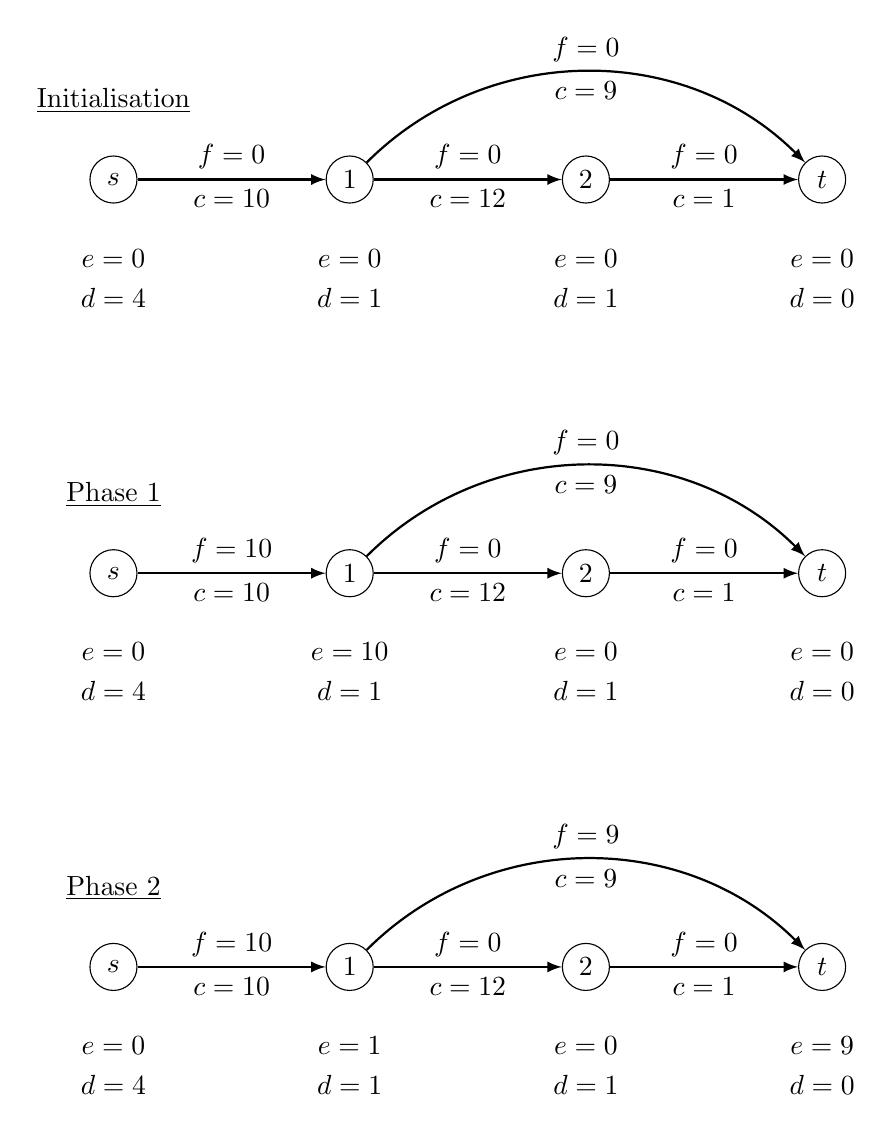
\begin{tikzpicture}[node distance=0.5cm]
			\tikzset{noeud/.style={circle, draw=black, minimum size=17pt, inner sep=1pt},
			fleche/.style={->,>=latex,thick}};


			\foreach \y/\f/\fl/\flo/\flot/\e/\ex/\text/\excd in {0/0/0/0/0/0/0/Initialisation/0,
				5/10/0/0/0/10/0/Phase 1/0, 10/10/0/0/9/1/0/Phase 2/9}{
					\node at (0, -1 * \y + 1) {\underline{\text}};
			\foreach \name/\x/\exc\dist in {s/0/0/4, 1/3/\e/1, 2/6/\ex/1, t/9/\excd/0}{
				\node[noeud] (\y-\name) at (\x, -1 * \y) {$\name$};
				\node (\y-e-\name) at (\x, -1 - \y ) {$e=\exc$};
				\node (\y-d-\name) [below of=\y-e-\name] {$d=\dist$};
			}

			\draw[fleche] (\y-s) -- node[above] {$f=  \f$} node[below] {$c=10$} (\y-1);
			\draw[fleche] (\y-1) -- node[above] {$f= \fl$} node[below] {$c=12$} (\y-2);
			\draw[fleche] (\y-2) -- node[above] {$f=\flo$} node[below] {$c= 1$} (\y-t);
			\draw[fleche] (\y-1) to[out=45, in=135]	node[above] {$f=\flot$} node[below] {$c= 9$} (\y-t);
		}

		\end{tikzpicture}
	\end{center}
	\caption{Exécution d'un algorithme n'utilisant que les méthodes de poussage}
	\label{ex_pouss}
\end{figure}

Le réétiquetage consiste à réévaluer la distance du n\oe ud débordant au n\oe ud puits de façon à ce
qu'il soit possible, après cette opération, d'effectuer une opération de poussage depuis ce n\oe ud.
Soit un n\oe ud excédentaire $i$ de distance $d_i$ et son $v_i$ son voisinage de sorte que $\forall v
\in v_i$, on a : $d_v \geq d_i$. La distance de $i$ doit être réévaluée afin de pouvoir évacuer
l'excédent de flot, il faut donc augmenter $d_i$ jusqu'à ce qu'un poussage puisse être réalisé ce
qui revient à fixer $d_i = 1 + \min(d_v), \quad v \in v_i$. 

L'algorithme générique se résume en deux étapes qui sont la procédure d'initialisation qui permet de
fournir une fonction de distance valide et de créer les premiers n\oe uds actifs en saturant les
arcs sortant de $s$ et une boucle agissant sur les n\oe uds débordants par poussage ou réétiquetage.

\begin{algorithm}
	\caption{Algorithme Générique}
	\label{algo_generic}
	\begin{algorithmic}[1]
			\STATE Initialisation() \\
			\WHILE{Il existe un noeud actif $i$}
				\STATE Pousser-Réétiqueter(i) 
			\ENDWHILE
	\end{algorithmic}
\end{algorithm}

\begin{algorithm}
	\begin{algorithmic}[1]
			\FOR{$i\ \in\ S$}
				\STATE Calculer la distance $d(i)$ en nombre d'arêtes de $i$ à $t$  
			\ENDFOR
			\FOR{$a$ $\in$ $A(s)$}
				\STATE $x(a)\ \leftarrow$ $c(a)$  
			\ENDFOR
			\STATE $d(s)\ \leftarrow |S|$ 
	\end{algorithmic}
	\caption{Procédure d'initialisation}
	\label{proc_init}
\end{algorithm}



La procédure Pousser-Réétiqueter appelle à quelques explications. La variable $p$ est un booléen
permettant de déterminer si l'algorithme a effectué une opération de poussage, si ce n'est pas la
cas, la procédure effectue un réétiquetage. La variable $f$ quant à elle permet de déterminer s'il
s'agit là de la première itération, afin de pouvoir initialiser correctement $m$ (qui est utilisé
pour rechercher le plus petit des voisins du n\oe ud effectuant l'algorithme).

\begin{algorithm}
	\begin{algorithmic}[1]
			\STATE $p \leftarrow \FALSE$ 
			\STATE $f \leftarrow \TRUE$  
			\FOR{$j \in A(i)$}
				\IF{$(i,j)$ est une arête acceptable}
					\STATE $x(i,j) \leftarrow \min(e(i), r(i,j))$  
					\STATE $p \leftarrow \TRUE$ 
					\STATE BREAK
				\ELSIF {$p = \FALSE$ \AND $d(i) < d(j)$}
					\IF {$r(i,j) > 0$ \AND $f = \TRUE$}
						\STATE $m \leftarrow d(j) + 1$ 
						\STATE $f \leftarrow \FALSE $
					\ELSIF {$r(i,j) > 0$}
						\STATE $m \leftarrow \min(m, d(j) + 1) $
					\ENDIF
				\ENDIF
			\ENDFOR
			\IF{$p = \FALSE$}
				\STATE $d(i) \leftarrow m$ 
			\ENDIF
		\end{algorithmic}
	\caption{Procédure Pousser-Réétiqueter}
	\label{proc_pousreet}
\end{algorithm}



Il sera démontré plus loin que cet algorithme s'exécute en $O(n^2m)$~\cite{gold88}.

\subsection{Validité}

\begin{thrm}
	L'algorithme de préflot générique se termine~\cite{introalg}.
\end{thrm}

Pour montrer que l'algorithme de préflot générique résout le problème du flot maximum, Nous allons démonter que s'il se termine, Alors le préflot $f$ calculé est un flot maximum!.\\

\textbf{Passage par les opérations de poussage et réétiquetage:}  

Considérons un graphe $G = (S,A)$ de source $s$ et de puits $t$, un préflot $f$ et une fonction de
distance valide $d$. Soit $u$ un sommet de $G$, on a alors :

\begin{lemma}
	\label{increase_distance}
  Si $u$ est débordant, alors il peut être soumis à une opération soit de poussage, soit de
	réétiquetage.  
\end{lemma}   
\textbf{Preuve} \\
Soit ($u$,$v$) un arc résiduel quelconque, donc on a $d(u)\leq d(v)+1$ car $d$ est une fonction  de
distance . Si une opération de poussage ne peut s'appliquer à $u$, alors pour tous les arcs
résiduels $(u,v)$, on doit avoir $d(u)< d(v)+1$, ce qui implique que $d(u)\leq d(v)$. Donc une
opération de réétiquetage peut être appliqué à $u$.\\

\textbf{Retour à $d$ la fonction de distance:}\\
\begin{lemma}
	\label{residual_path}
	A n'importe quelle itération de l'algorithme, la fonction $d$ est une fonction de distance valide.
\end{lemma}  
\textbf{Preuve} \\
  On raisonne par récurrence sur le nombre d'opérations élémentaires effectuées.
  Après l'initialisation au départ, $d$ est bien une fonction de distance valide.\\

	Obeservons l'influence des opérations sur cette dernière :\begin{itemize}
  
  \item Le réétiquetage:
  Comme nous l'avons déjà vu.
  On assure que si $d$ est une fonction de distance valide, alors elle le restera après une opération de réétiquetage de $u$.
	Considérons un arc $(u,v) \in A_f, \quad u, v \not = s, t$, par définition, on a $d(u) \leq d(v) + 1$, envisageons deux
	cas : \begin{enumerate}
	\item $d(u) \geq d(v)$ : l'opération de réétiquetage appliquée à $u$ augmentera la valeur de
	$d(u)$ d'au moins 1 et donc après l'opération, on aura toujours $d(u) \geq d(v)$
	\item $d(v) = d(u) + 1$ : l'opération de réétiquetage appliquée à $u$ augmentera la valeur de
	$d(u)$ d'au moins 1 et donc après l'opération, on aura toujours $d(u) \geq d(v)$
	\end{enumerate}
	L'opération de réétiquetage conserve la validité de la fonction de distance.
  
	\item Le poussage :
	Considérons les sommets $u$ et $v$ tels que $u$ pousse vers $v$. Nous envisagerons deux cas :
	\begin{enumerate}
	\item le poussage crée l'arête $(v,u)$ dans $A_f$ : par définition du poussage, $d(u) = d(v) + 1$
	donc $d$ est toujours valide
	\item le poussage supprime l'arc $(u,v)$ dans $A_f$ : la contrainte correspondante est supprimée
	et donc $d$ est toujours un fonction de distance valide
	\end{enumerate}
	\end{itemize}
 
\begin{lemma}
	\label{borne_reetiq}Il n'existe aucun chemin allant de la source $s$ au puits $t$ dans le réseau résiduel $G_f$.
\end{lemma} 

\textbf{Preuve} \\
Supposons le contraire, c'est-à-dire qu'il existe un chemin élémentaire $µ$ $=$\{$v_0$,....,$v_k$\} avec $v_0$ $=$ $s$ et $v_k$ $=$ $t$ de $s$ vers $t$ dans $A_f$.
$µ$ élémentaire donc $k$ $<$ $|$ $s$ $|$
Soit $i$ $=$\{0,1,...,$k$ $-$1\}, l'arc ($v_i$,$v_{i+1}$)$\in$ $A_f$. Comme $d$ est une fonction de distance $d$($v_i$)$\leq$ $d$($v_{i+1}$)$+$1 encore pour $i$ $=$\{0,1,...,$k$ $-$1\}, en appliquant ces inégalités sur tout le chemin $µ$, on aura
$d$($s$)$\leq$ $d$($t$)$+$ $k$. Mais comme $d$($v_k$)$=$ $d$($t$)$=$0, on obtient 
$d$($s$)$=$ $k$ $<$ $|$ $s$ $|$, ce qui contredit la contrainte $d$($s$)$=$ $|$ $s$ $|$ pour une fonction de distance \\

\begin{thrm}
Si l'algorithme de préflot se termine, Alors le préflot $f$ calculé est un flot maximum.
\end{thrm}

\textbf{Preuve} \\
 Regardons la boucle 'Tant que' dans l'algorithme préflot générique A chaque exécution de test de cette boucle, $f$ est un préflot.
 
 \textbf{Initialisation:} Initialiser-préflot fait de $f$ est un préflot.\\ 
 
 \textbf{Conservation:} Les seules opérations faites dans la boucle 'tant que' sont soit l'opération
 de poussage, soit celle de réétiquetage.  
 L'opération de réétiquetage modifie uniquement la distance du sommet sur lequel elle est appliquée,
 donc elle ne modifie pas la valeur du préflot. De plus, si $f$ est un préflot avant poussage il le
 reste après et donc, les opérations conserve le préflot $f$.

 
 \textbf{Terminaison:}A la fin de l'exécution de l'algorithme, chaque sommet de
$S$-\{$s$,$t$\} doit avoir un excédent nul, en effet d'après les lemmes \ref{increase_distance} et
\ref{residual_path} et l'invariant selon lequel $f$ est toujours un préflot, il n'y a pas de sommets
débordants, or comme $d$ est une fonction de distance valide, le lemme \ref{borne_reetiq} nous dit
qu'il n'y a pas de chemins entre la source $s$ et le puits $t$ dans le réseau résiduel $A_f$.
 Alors d'après le théorème du flot maximum et la coupe minimum le préflot $f$ calculé est un flot maximum.  


\section{Les algorithmes dérivés}

Nous présenterons dans cette section, les différents algorithmes reposant sur l'algorithme générique
présenté précédemment. Pour la totalité d'entre eux, il s'agit de chercher à réaliser un choix
judicieux pour l'examen des n\oe uds débordants.

\subsection{L'algorithme FIFO}

L'algorithme FIFO, utilise une file afin de gérer l'ordre des n\oe uds actifs à traiter : au moment
ou un sommet du graphe devient débordant, celui-ci est placé dans une file, dont la politique de
traitement est du type \emph{First In First Out}. 

A chaque examen, l'algorithme réalise des opérations de poussage tant que celles-ci sont possibles et
tant que le n\oe ud $i$ examiné est débordant. Si, lorsqu'il n'existe plus d'arêtes acceptables,
$e(i)$ est toujours supérieur à $0$, l'algorithme réalise donc un réétiquetage et place à nouveau
$i$ dans la file des sommets à examiner. L'initialisation de l'algorithme est la procédure
principale restent les mêmes que l'algorithme générique.

Ce choix permet une amélioration de la complexité de l'algorithme générique en
$O(n^3)$~\cite{ahuj93}.

\subsection{L'algorithme High label}

Il existe des graphes pour lesquels, l'algorithme FIFO est très lent. On peut par exemple citer
celui décrit figure \ref{bad_fifo}.

\begin{figure}
\begin{center}
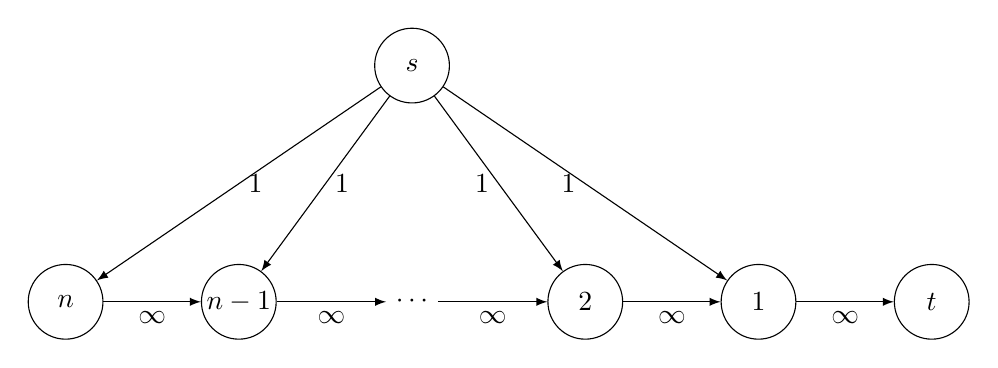
\begin{tikzpicture}[node distance=2.2cm]
\tikzset{n/.style={circle, draw=black, minimum size=27pt, inner sep=1pt}, 
f/.style={->, >=latex}};

\node[n] (s) at (4.4, 3) {$s$};
\node[n] (n0) at (0, 0) {$n$};
\node[n] (n1) [right of=n0] {$n-1$};
\node[right of=n1] (point) {$\cdots$};
\node[n, right of=point] (2) {$2$};
\node[n, right of=2] (1) {$1$};
\node[n, right of=1] (t) {$t$};

\foreach \x/\pos in {n0/right, n1/right, 2/left, 1/left} {
	\draw[f] (s) to node[\pos] {$1$} (\x);
}

\draw[f] (n0) to node[below] {$\infty$} (n1);
\draw[f] (n1) to node[below] {$\infty$} (point);
\draw[f] (point) to node[below] {$\infty$} (2);
\draw[f] (2) to node [below] {$\infty$} (1);
\draw[f] (1) to node [below] {$\infty$} (t);

\end{tikzpicture}
\end{center}
\caption{Exemple de graphe mettant en défaut l'algorithme FIFO}
\label{bad_fifo}
\end{figure}

En effet, lors de l'initialisation de ce dernier, les n\oe uds vont être placés en file d'attente
selon l'ordre de traitement des arêtes sortant de $s$. Si celui ci se fait par ordre
lexicographique, le sommet $1$ sera placé dans la file en premier puis le $2$ et ainsi de suite
jusqu'au sommet $n$. L'examen se fera donc dans cet ordre, on s'aperçoit alors que $1$ pousse son
excédent vers $t$, puis $2$ pousse son excédent vers $1$ et ainsi de suite jusqu'au n\oe ud $n$
poussant vers $n-1$.
Puis le traitement recommence à partir de $1$ jusque $n-1$, puis de $1$ jusque $n-2$, etc... On
dénombre alors $n!$ opérations.

Le principe de l'algorithme High Label est de choisir pour l'examen, le n\oe ud ayant la distance la
plus grande, de lui appliquer le plus grand nombre de poussage et de le réétiqueter si besoin est.
L'algorithme effectue, sur le graphe représenté figure \ref{bad_fifo}, seulement $n$ opérations.
Nous démontrerons que la complexité de cet algorithme s'en voit améliorée pour atteindre du
$O(n^2\sqrt{m})$~\cite{ahuj93}.
